\documentclass{beamer}
\usetheme{Darmstadt}
\usepackage{CJKutf8}

\usepackage[utf8]{inputenc}
\usepackage[OT1, T2A]{fontenc}
\usepackage{fontspec}
\usepackage[normalem]{ulem}

\usepackage{graphicx}
\usepackage{tikz}
\usetikzlibrary{quantikz}
\usepackage{braket}

\usepackage{xcolor}
\usepackage{pgfplots}
\usepackage{tikz}

\begin{document}
    \begin{frame}{Quantum S-DES Implementation}
        Initially, 34 explicit qubits were used in total.
        \begin{itemize}
            \item 10 qubits for input key
            \item 1 qubit for making an encryption oracle
            \item 8 qubits for (intermediate) plaintext
            \item 8 qubits for expanded plaintext
            \item 4 qubits for storing S-Box result
            \item 3 qubit for S-Box ancilla
        \end{itemize}
        S-DES implementation is written in Microsoft Q\#. Will it run?
    \end{frame}

    \begin{frame}{Quantum S-DES Implementation}
        Yes, and no.
        \begin{figure}[h]
            \centering
            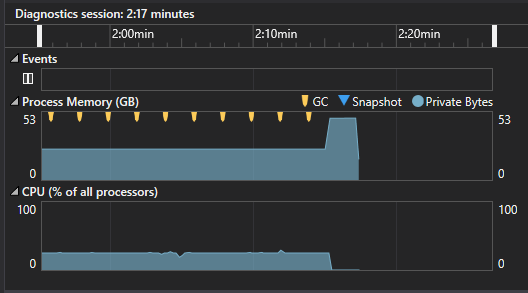
\includegraphics[height=0.5\textheight]{./Images/Qsharp-SDES-memory-error-2.png}
        \end{figure}
        After allocating 48GB of RAM, \texttt{System.Runtime.InteropServices.SEHException} was raised, indicating an out-of-memory error.
    \end{frame}

    \begin{frame}{Quantum S-DES Implementation}
        Reducing the number of qubits was necessary...!
        \begin{itemize}
            \item 10 qubits for input key
            \item 1 qubit for making an encryption oracle
            \item 8 qubits for (intermediate) plaintext
            \item \only<1>{8 qubits for expanded plaintext} \only<2->{{\color{gray}\sout{8 qubits for expanded plaintext}}}
            \item \only<1-2>{4}\only<3->{{\color{gray}\sout{4}} 2} qubits for storing S-Box result
            \item \only<-3>{3 qubits for S-Box ancilla} \only<4>{{\color{gray}\sout{3 qubits for S-Box ancilla}}}
        \end{itemize}
        \onslide<2-> We can directly use plaintext qubits to create result qubits from S-Box. After then we can undo all the operations (permutation, \textit{etc.}) which altered plaintext.

        \onslide<3->Additionally, each S-Box operation is independent. Thus we can reuse S-box result qubits after re-initialization.

        \onslide<4->Finally, redundant S-Box ancilla qubits were removed.
    \end{frame}


    \begin{frame}{Quantum S-DES Implementation}
        However, applying Grover's was not simple as it looked
        \begin{itemize}
            \item The oracle should be adjoint, but original version includes measurement (in result ciphertext and S-Box)
            \item How to create an oracle qubit rather than measuring the result ciphertext?
            \begin{itemize}
                \item perform CNOT gate 8 times (with 7 more qubits) : infeasible
                \item Microsoft Q\#'s \texttt{Controlled} functor : doable
            \end{itemize}
            \item Similar to S-Box Controlling
            \item S-Box also required measurement initially, but change to forementioned circuit
        \end{itemize}
        Result : reversible S-DES oracle.

    \end{frame}

    \begin{frame}{Quantum S-DES Implementation}
        \begin{figure}
            \centering
            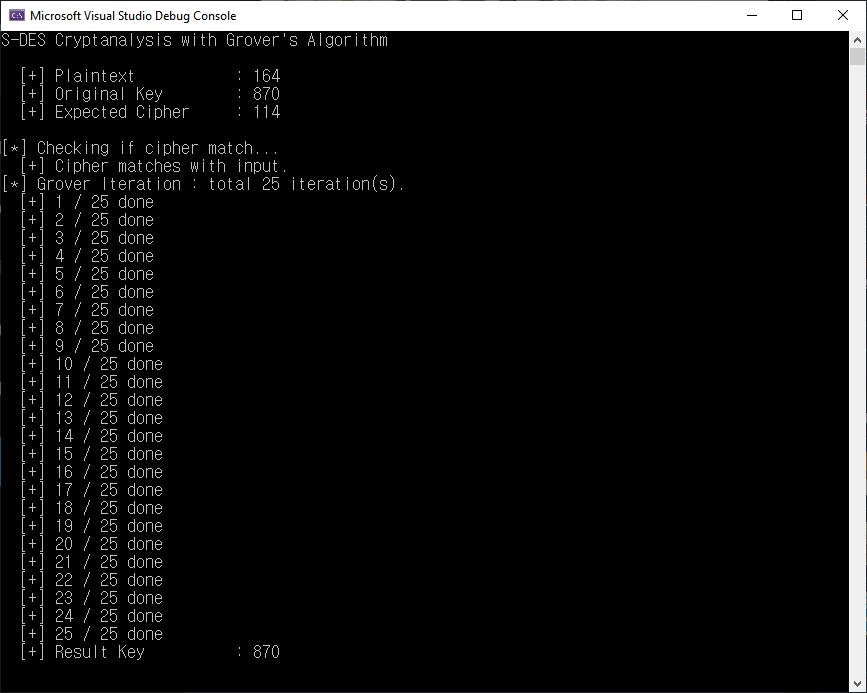
\includegraphics[height=0.5\textheight]{./Images/Qsharp-SDES-Grover-k1.png}
        \end{figure}
        Expected key matched with original key (with runtime 1 min 12 sec, performing each S-DES encryption within 2-3s on average).
    \end{frame}
\end{document}